\documentclass[10pt,twocolumn]{article}
% Form nach A. Suleman, "Optimal lattices for a three-body power-law energy" (Preprint 2026): zweispaltig, Journal-Kopf, Inline-Abstract.
\usepackage[utf8]{inputenc}\usepackage[T1]{fontenc}\usepackage{lmodern}\usepackage{microtype}
\usepackage[english]{babel}\usepackage[a4paper,top=2.3cm,bottom=2.3cm,left=1.8cm,right=1.8cm,columnsep=0.65cm]{geometry}
\usepackage{amsmath,amssymb,amsthm}\usepackage{graphicx}\usepackage{booktabs,array,calc}
\usepackage[font=small,labelfont=bf,labelsep=space,figurename=Fig.]{caption}
\usepackage{fancyhdr}\usepackage{titlesec}\usepackage[hidelinks]{hyperref}\usepackage[capitalise,noabbrev]{cleveref}\usepackage{newunicodechar}
\titleformat{\section}{\normalfont\large\bfseries}{\thesection}{0.6em}{}\titleformat{\subsection}{\normalfont\bfseries}{\thesubsection}{0.6em}{}
\titlespacing*{\section}{0pt}{1.6ex plus .5ex}{0.9ex}\titlespacing*{\subsection}{0pt}{1.2ex plus .4ex}{0.6ex}
\newunicodechar{η}{\ensuremath{\eta}}
\newunicodechar{Δ}{\ensuremath{\Delta}}
\newunicodechar{σ}{\ensuremath{\sigma}}
\newunicodechar{μ}{\ensuremath{\mu}}
\newunicodechar{≥}{\ensuremath{\geq}}
\newunicodechar{≤}{\ensuremath{\leq}}
\newunicodechar{×}{\ensuremath{\times}}
\newunicodechar{→}{\ensuremath{\to}}
\newunicodechar{≈}{\ensuremath{\approx}}
\newunicodechar{−}{\ensuremath{-}}
\newunicodechar{·}{\ensuremath{\cdot}}
\newunicodechar{∈}{\ensuremath{\in}}
\newunicodechar{…}{\ensuremath{\ldots}}
\newunicodechar{²}{\ensuremath{^{2}}}
\newunicodechar{³}{\ensuremath{^{3}}}
\newunicodechar{√}{\ensuremath{\surd}}
\newunicodechar{±}{\ensuremath{\pm}}
\newunicodechar{⁻}{\ensuremath{^{-}}}
\newunicodechar{¹}{\ensuremath{^{1}}}
\newunicodechar{₀}{\ensuremath{_{0}}}
\newunicodechar{₁}{\ensuremath{_{1}}}
\newunicodechar{₂}{\ensuremath{_{2}}}
\newunicodechar{α}{\ensuremath{\alpha}}
\newunicodechar{β}{\ensuremath{\beta}}
\newunicodechar{γ}{\ensuremath{\gamma}}
\newunicodechar{ε}{\ensuremath{\varepsilon}}
\newunicodechar{τ}{\ensuremath{\tau}}
\newunicodechar{ν}{\ensuremath{\nu}}
\newunicodechar{∞}{\ensuremath{\infty}}
\newunicodechar{≠}{\ensuremath{\neq}}
\newunicodechar{π}{\ensuremath{\pi}}
\newunicodechar{λ}{\ensuremath{\lambda}}
\newunicodechar{ρ}{\ensuremath{\rho}}
\newunicodechar{θ}{\ensuremath{\theta}}

\providecommand{\tightlist}{\setlength{\itemsep}{0pt}\setlength{\parskip}{0pt}}
\newtheorem{theorem}{Theorem}\newtheorem{proposition}{Proposition}\newtheorem{lemma}{Lemma}\newtheorem{corollary}{Corollary}
\theoremstyle{definition}\newtheorem{definition}{Definition}\newtheorem{example}{Example}
\newtheorem{observation}{Numerical observation}\theoremstyle{remark}\newtheorem{remark}{Remark}
\pagestyle{fancy}\fancyhf{}\renewcommand{\headrulewidth}{0pt}
\fancyhead[L]{\small Preprint (2026)}\fancyhead[R]{\small C. Ji et al.: Eleven exactly certified violations of the proofreading bound ...}\fancyfoot[C]{\small\thepage}
\begin{document}
\twocolumn[{%
\noindent{\small Preprint}\\[-1pt]
\noindent{\small\itshape Biological Physics}\\[12pt]
\noindent{\LARGE\bfseries\raggedright Eleven exactly certified violations of the proofreading bound $e^{-2\Delta}$ among 88 two-bound-state networks\par}\vspace{10pt}
\noindent{\large Colin Ji, Laurenz Thümmler, Noah Schittenhelm and Ali Suleman}\\[3pt]
\noindent{\small ETH Zürich, Switzerland}\\[2pt]
\noindent{\small Preprint, October 2026}\par\vspace{16pt}
}]
\thispagestyle{plain}
\noindent\textbf{Abstract} We ask whether the Hopfield error bound of kinetic proofreading holds universally for Markov networks with two bound states and fuel-driven steps. For the linear Hopfield chain with \(n=2\), \(\eta \geq e^{-3\Delta}\) is proved for all positive rates and fuel potentials by a symbolic coefficient-positivity argument. The enumerated family has 88 admissible members. For 50 of them, \(\eta \geq e^{-2\Delta}\) is proved symbolically; 11 have exact rational-arithmetic certificates of violation, with \(\eta\) down to 1.386398e-12; 27 remain open. Hence \(e^{-2\Delta}\) is violated by 11 of these networks. The classification is computer-assisted: the bounds are symbolic, and the violations are exact rational certificates at specific rates. Whether the 27 open members obey the bound, and which structural feature causes violations, remains open.
\par\medskip
\noindent\textbf{Keywords} kinetic proofreading $\cdot$ Hopfield bound $\cdot$ error rate $\cdot$ exact certificates $\cdot$ Markov networks $\cdot$ entropy production\par\medskip
\emph{Author: alizema700@gmail.com}

\section{Introduction}\label{introduction}

Kinetic proofreading increases specificity beyond what free-energy differences or kinetic barriers alone allow, if the reaction is strongly but nonspecifically driven \cite{Hopfield19744135}. The ultimate accuracy of error-correcting pathways is set by the displacement from equilibrium of the driving nucleoside triphosphates \cite{Ehrenberg19800636}. Several checking steps reach a given accuracy at lower dissipation than a single step \cite{Ehrenberg19800636}. Pareto fronts for energy-relay proofreading yield trade-off relations and scaling laws \cite{Berx20240232}, and a dynamical phase transition has been reported in the mixed regime \cite{Berx20240232}. In the generalized Hopfield model, more proofreading steps give better trade-offs \cite{Chiuchiu2023c757}, and the scaling relations were studied numerically \cite{Chiuchiu2023c757}. A kinetically controlled bound on error for proofreading networks has been derived \cite{Yu20220883}, and experimental systems have been compared with it \cite{Yu20220883}. Asymptotic scaling analyses of arbitrary networks, inspired by Hopfield's treatment, have also been given \cite{Wong201738v1}.

The open question is whether the Hopfield bound \(\eta \geq e^{-(n+1)\Delta}\) is a universal limit for all networks with a fixed number of bound states, or whether topologies with fuel-driven discard pathways break it. The question is hard because the topology space is combinatorial and the rate space is high-dimensional, and numerical optima cannot establish a bound. A lower bound must hold for all rates. A violation must be exact, which excludes rounding artefacts. We therefore pair symbolic positivity proofs for bounds with exact rational certificates for violations.

\textbf{Summary of results.}

\begin{itemize}
\tightlist
\item
  Theorem 1 shows that the family with two bound states has 88 admissible members, of which 50 obey \(\eta \geq e^{-2\Delta}\), 11 have certified violations and 27 are open.
\item
  Theorem 2 shows an exactly certified violation for fam2\_66, with \(\eta = 5.082802\)e-07.
\item
  Theorem 3 shows two further exact violations, fam2\_9 and fam2\_11.
\item
  Theorem 4 shows exact violations for 10 topologies jointly, which adds eight to those of Theorem 3.
\item
  The Hopfield-chain theorem shows that \(\eta \geq e^{-3\Delta}\) holds for the chain with \(n=2\) for all positive rates and fuel potentials.
\item
  The 50-topology theorem shows that \(\eta \geq 1/D^2\) is proved symbolically for 50 topologies of the family, where \(1/D^2\) is the bound \(e^{-2\Delta}\) of the classification.
\end{itemize}

\section{Setting}\label{setting}

All parameters are fixed by the model. The discrimination free-energy difference is \(\Delta = \ln 100\), so \(e^{\Delta} = 100\) and \(e^{-\Delta} = 0.01\). The wrong substrate W leaves bound states \(e^{\Delta}\) times faster than the right substrate R. Both substrates traverse the same Markov network, every edge has a reverse edge, and local detailed balance holds. Cycle affinities arise only from the fuel potential \(\mu \geq 0\) per fuel-driven activation and \(\mu_P \geq 0\) per product, both explored in \([0,20]\). Concentrations are absorbed into the binding rates. All rates, including derived reverse rates, lie in \([e^{-L}, e^{L}]\) with \(L = 10\). A network has at most 10 states (unbound states plus R and W copies of bound states). Rates are rounded to rationals with denominator at most \(10^6\) for exact certificates. The enumerated family has \(k=2\) bound states.

Observables are the error rate \(\eta = J_W/J_R\), the dissipation \(\sigma\) (entropy production per product, in \(kT\)), and the speed \(v = J_R\). We write \(D = e^{\Delta}\) and \(G = e^{\mu}\). The bound \(1/D^2\) of the proved family is the bound \(e^{-2\Delta}\) of the classification.

Four are degenerate (no net production possible, \(\eta = 0/0\)) and are excluded, leaving 88. Two certificate types are used:

\begin{itemize}
\tightlist
\item
  \textbf{(a)} exact reachability: rational rates satisfying all constraints with the stated inequalities;
\item
  \textbf{(b)} symbolic: \(\eta - B = N/D\) with all coefficients of \(N\) and \(D\) nonnegative, which proves \(\eta \geq B\) for all positive rates.
\end{itemize}

\section{Classification and certified violations}\label{classification-and-certified-violations}

\begin{theorem}[Classification of the two-bound-state family]
The bound \(e^{-2\Delta}\) is therefore violated by these 11 networks.
\end{theorem}

\emph{Certificate.} The counts were recomputed from the confirmed claims by the classification script. The counts 50, 11 and 27 sum to the family size of 88. Novelty status: not found in the literature search for the classification and the counterexamples.

\begin{theorem}[Violation in fam2\_66]
For the topology fam2\_66 there exist rational rates in \([e^{-10}, e^{10}]\) satisfying local detailed balance such that simultaneously \(\eta \leq 0.0001\) and \(v \geq 0.0001\).
\end{theorem}

\emph{Certificate.} The topology has binding to C0, a fuel-driven conversion C0 to C1, a fuel-driven discard from C1, and product formation from C1. Exact reachability (a) gives \(\eta = 5.082802\)e-07, \(\sigma = 8.341626\,kT\) per product and \(v = 1.4746\)e-03. Novelty status: not found in a targeted search of 48 abstracts on 2026-10-04.

\begin{theorem}[Violations in fam2\_11 and fam2\_9]
For each of the two topologies fam2\_11 and fam2\_9 there exist rational rates in \([e^{-10}, e^{10}]\) satisfying local detailed balance with \(\eta \leq 0.0001\).
\end{theorem}

\emph{Certificate.} Certificate (a), checked in exact arithmetic for each case, passed for 2/2 cases. Novelty status: not found in a targeted search of 42 abstracts on 2026-10-04.

\begin{theorem}[Further violations]
For each of the 10 topologies fam2\_11, fam2\_35, fam2\_39, fam2\_41, fam2\_43, fam2\_45, fam2\_58, fam2\_67, fam2\_75 and fam2\_9 there exist rational rates in \([e^{-10}, e^{10}]\) satisfying local detailed balance with \(\eta \leq 0.0001\).
\end{theorem}

\emph{Certificate.} Certificate (a) was checked exactly for each case and passed for 10/10 cases. Two of these, fam2\_9 and fam2\_11, are already covered by the preceding theorem. Novelty status: not checked.

The table lists the exact error rates of the certified violations. All are strictly below \$e\^{}\{-2\Delta\} = \$ 1e-4.

\begin{table}[t]\centering\footnotesize
\caption{Exact error rates of the certified violations (rational rates, exact arithmetic).}
\begin{tabular}{@{}lll@{}}
\toprule
Topology & \(\eta\) (exact) & Source \\
\midrule
fam2\_9 & 2.000856e-05 & proofreading-R12 \\
fam2\_11 & 4.417288e-05 & proofreading-R12 \\
fam2\_35 & 1.074798e-06 & proofreading-O14 \\
fam2\_39 & 1.010274e-06 & proofreading-O14 \\
fam2\_41 & 1.287193e-06 & proofreading-O14 \\
fam2\_43 & 1.386398e-12 & proofreading-O14 \\
fam2\_45 & 1.591024e-06 & proofreading-O14 \\
fam2\_58 & 7.272608e-08 & proofreading-O14 \\
fam2\_66 & 5.082802e-07 & proofreading-R4 \\
fam2\_67 & 4.098578e-07 & proofreading-O14 \\
fam2\_75 & 1.142234e-06 & proofreading-O14 \\
\bottomrule
\end{tabular}
\end{table}


\begin{remark}[Status of the computer-assisted parts]
All statements in this article are computer-assisted. Type-(a) certificates rest on exact rational arithmetic with rates rounded to rationals of bounded denominator. Type-(b) certificates rest on exact symbolic expansion and a check that all coefficients are nonnegative. The trusted base is the domain verifier, which passes its self-test with 18 of 18 cases (true, false, boundary and rule-violating cases). The numerical optimiser that finds candidate rates is not part of the trusted base, since only the exact check of the returned rationals counts. A third party re-runs every certificate with \texttt{python\ -m\ asd.recheck\ proofreading} and rebuilds the paper with \texttt{python\ -m\ asd.paper\ -\/-domain\ proofreading}.
\end{remark}

\section{Proved bounds}\label{proved-bounds}

\begin{theorem}[Hopfield bound for the chain with $n=2$]
For the linear Hopfield chain hopfield\_n2, \(\eta \geq e^{-3\Delta}\) holds for all positive rates and all fuel potentials \(\mu, \mu_P \geq 0\) (with \(D = e^{\Delta}\), \(G = e^{\mu}\)).
\end{theorem}

\emph{Proof.} Symbolic positivity (certificate (b)): \(\eta - e^{-3\Delta} = N/D\) with \(N\) and \(D\) having 1374 and 2048 terms respectively, and all coefficients nonnegative (check returned True in 6.8 s). The proof is independent of the rate range. Novelty status: not found in a targeted search of 40 abstracts on 2026-10-04. The novelty check classifies the chain bound as a reproduction of the Hopfield bound, treated here rigorously.

\begin{theorem}[Proved bound for 50 topologies]
For 50 topologies of the verifier-generated family with at most two bound states (one unbound state, edge catalogue of the model), \(\eta \geq 1/D^2\) holds for all positive rates and fuel potentials. This is the bound \(e^{-2\Delta}\) of the classification.
\end{theorem}

\emph{Proof.} Symbolic certificate (b), with the bound proved for 50/50 members of the complete list. Novelty status: not found in a targeted search of 48 abstracts on 2026-10-04.

\section{Supporting statements and examples}\label{supporting-statements-and-examples}

\begin{proposition}[Smaller sublists]
For 3 topologies of the verifier-generated family with at most two bound states, \(\eta \geq 1/D^2\) holds for all positive rates and fuel potentials (certificate (b), symbolic).
\end{proposition}

\emph{Proof.} Symbolic certificate (b), 3/3 members proved, once for the largest justified sublist and once for the question whether going below \(e^{-2\Delta}\) requires a fuel-driven discard exit at the product state. Novelty status: not found in targeted searches of 41 and 35 abstracts respectively on 2026-10-04. Both lists are superseded by the 50-topology theorem.

\begin{proposition}[Consistency of the count]
For 50 topologies of the verifier-generated family, \(\eta \geq 1/D^2\) holds for all positive rates and fuel potentials (certificate (b), symbolic), consistent with the classification.
\end{proposition}

\emph{Proof.} The certificate proved the bound for 50/50 members. Novelty status: not checked.

The following exact points of the one-stage Hopfield chain (hopfield\_n1) are certificates (a) of exact reachability. They are existence statements, not bounds.

\begin{example}[Reachability at moderate dissipation]
For hopfield\_n1 there exist rational rates in \([e^{-10}, e^{10}]\) satisfying local detailed balance with simultaneously \(\eta \leq 0.0004\), \(\sigma \leq 6.0\,kT\) per product and \(v \geq 0.001\).
\end{example}

\emph{Certificate.} Exact rational reachability check gives \(\eta = 3.650169\)e-04, \(\sigma = 6.000000\,kT\), \(v = 1.0417\)e-01. Novelty status: not found in a targeted search of 62 abstracts on 2026-10-04. The novelty check classifies reachable points of the chain as qualitatively known, here exact.

\begin{example}[Reachability with $\eta \leq 0.01$]
For hopfield\_n1 there exist rational rates in \([e^{-10}, e^{10}]\) satisfying local detailed balance with simultaneously \(\eta \leq 0.01\) and \(v \geq 0.001\).
\end{example}

\emph{Certificate.} Exact rational reachability check gives \(\eta = 5.909757\)e-03, \(\sigma = 3.998555\,kT\), \(v = 7.1214\)e-03. Novelty status: not found in a targeted search of 45 abstracts on 2026-10-04.

\begin{example}[Reachability at very low dissipation]
For hopfield\_n1 there exist rational rates in \([e^{-10}, e^{10}]\) satisfying local detailed balance with simultaneously \(\eta \leq 0.00012\) and \(\sigma \leq 0.2\,kT\) per product.
\end{example}

\emph{Certificate.} Exact rational reachability check gives \(\eta = 1.095823\)e-04, \(\sigma = 0.006292\,kT\), \(v = 9.1487\)e-09. The speed at this point is very small. Novelty status: not found in a targeted search of 49 abstracts on 2026-10-04.

\begin{example}[Reachability with a speed floor]
For hopfield\_n1 there exist rational rates in \([e^{-10}, e^{10}]\) satisfying local detailed balance with simultaneously \(\eta \leq 0.0002\), \(\sigma \leq 10\,kT\) per product and \(v \geq 0.001\).
\end{example}

\emph{Certificate.} Exact rational reachability check gives \(\eta = 1.189200\)e-04, \(\sigma = 4.271813\,kT\), \(v = 1.0000\)e-03. Novelty status: not found in a targeted search of 37 abstracts on 2026-10-04.

\section{Discussion}\label{discussion}

The chain bound is the Hopfield bound for two proofreading stages, proved for all positive rates. The classification shows that the corresponding statement for \(e^{-2\Delta}\) fails for 11 members of the family with two bound states. Fam2\_66 has a fuel-driven discard from C1 and exhibits a violation. We did not establish that such pathways are necessary, so this is an observation about one topology and not a criterion. The symbolic bound for all positive rates in the sublist question covers only 3 topologies.

The violations are exact existence statements at specific rational rates. They give no phase diagram and no information on the Pareto front of the violating networks. The operating points have high dissipation, for instance \(\sigma = 8.341626\,kT\) per product at \(v = 1.4746\)e-03 for fam2\_66. Whether such points are generic is not addressed. The 27 open members are neither proved nor refuted, so the classification is incomplete.

\textbf{What did not work.} First, the attempt to prove the bound for the sublist without a fuel-driven discard exit produced no verified claim, because of verifier errors that were fixed later. Second, the search for further violations among the open topologies passed certificate (a) for all but one of the cases. The remaining case, fam2\_13, failed because a rate left the allowed window (\(|\log k| = 10.06\), derived reverse rates included).

Open questions:

\begin{enumerate}
\def\labelenumi{(\roman{enumi})}
\item
  What is the status of the 27 open topologies: does each obey \(\eta \geq e^{-2\Delta}\) or violate it?
\item
  Is there a structural criterion on the topology that separates the 50 proved members from the 11 violating ones?
\item
  Does fam2\_13 admit a violation with all rates, including derived reverse rates, inside \([e^{-10}, e^{10}]\)?
\end{enumerate}

\section*{Declarations}\label{declarations}
\addcontentsline{toc}{section}{Declarations}

\textbf{Affiliation} No institutional affiliation is given in the author line; contact: alizema700@gmail.com.

\textbf{Acknowledgements} Computations, literature searches and parts of the manuscript were prepared with an automated verifier-gated laboratory built on the AI system Claude (Anthropic). Every statement was accepted only after verification by code. The authors are responsible for the content.

\textbf{Code and data availability} Repository https://github.com/alizema700/Daddys-Project, branch claude/probatum-mcp, directory projects/omni\_proofreading. All certificates are reproduced with \texttt{python\ -m\ asd.recheck\ proofreading}, and the paper is rebuilt with \texttt{python\ -m\ asd.paper\ -\/-domain\ proofreading}.

\textbf{Competing interests} None.

\appendix

\section{Numerical methods and error control}\label{numerical-methods-and-error-control}

\textbf{Certificate types.} Type (a) fixes rational rates (denominator at most \(10^6\)) and evaluates \(\eta\), \(\sigma\) and \(v\) exactly, so that the inequalities are checked without rounding. A rate outside \([e^{-10}, e^{10}]\) is rejected, including derived reverse rates. Type (b) expands \(\eta - B\) as \(N/D\) and checks that all coefficients are nonnegative.

\textbf{Trusted base and self-test.} The verifier passes its self-test with 18 of 18 cases. Re-running: \texttt{python\ -m\ asd.recheck\ proofreading}.

\textbf{Counter-checks as consistency tests.} A symbolic attempt to prove \(\eta \geq 1.2\,e^{-2\Delta}\) at the claimed point of the low-dissipation example fails (137 and 167 terms, not all coefficients nonnegative). Attempts to prove the bound \(1/D^2\) for the violating members fail (0/3 and 0/8 proved). For the parameter set examined in the first reachability example, the same point remains admissible at larger dissipation budgets, which is incompatible with a reported jump of the front at that point. An independent search for \(n=2\) found \(\eta_{\min} = 3.1387\)e-05 at \(\sigma = 2665.585\), not the lower value tested. A further \(n=2\) check gave \(\eta = 4.879638\)e-06 at \(\sigma = 172.281249\).

\textbf{Workflow.} The laboratory ran 16 rounds with 14 verified statements and 2 negative results, each round preregistered before the experiment. The preregistration (commit 6184672) preceded the first run, and later additions are dated. The success criterion of at least 5 counterexamples in one round was missed: 2 were found in round 12, 3 in total. Round 12 passed certificate (a) for 2/2 cases. The attempts on the discard-exit question were made by the agents sparsam/haiku, numeriker/haiku, skeptiker/sonnet and theoretiker/sonnet, and one further search by omnigent:researcher.

\textbf{Literature search and red-team.} The search retrieved 2752 sources, screened 2502, and found 158 results with a code-confirmed verbatim quote; all 11 classic searches had hits. Red-team counter-checks: 29 in total, 5 passed, 12 did not pass, 12 not executable. The novelty statuses in the text come from targeted searches per result.

\section{Provenance of the statements}\label{provenance-of-the-statements}

The provenance table mapping every statement to its evidence follows; it is generated automatically.

{\def\LTcaptype{none} % do not increment counter
\begin{table*}[t]\centering\footnotesize
\begin{tabular}{@{}
  >{\raggedright\arraybackslash}p{(\linewidth - 4\tabcolsep) * \real{0.3333}}
  >{\raggedright\arraybackslash}p{(\linewidth - 4\tabcolsep) * \real{0.3333}}
  >{\raggedright\arraybackslash}p{(\linewidth - 4\tabcolsep) * \real{0.3333}}@{}}
\toprule
\begin{minipage}[b]{\linewidth}\raggedright
Statement
\end{minipage} & \begin{minipage}[b]{\linewidth}\raggedright
Evidence (claim ids)
\end{minipage} & \begin{minipage}[b]{\linewidth}\raggedright
Level
\end{minipage} \\
\midrule
Section: Introduction & C-fakt-fam66, C-fakt-familie, C-fakt-klassifikation, C-proofreading-O14, C-proofreading-R11, C-proofreading-R12, C-proofreading-R4, C-proofreading-R9 & computed\_rigorous \\
Section: Setting & C-fakt-familie, C-fakt-klassifikation, C-modell, C-proofreading-R11, C-proofreading-R9 & computed\_rigorous \\
Theorem 1 (Classification of the two-bound-state family) & C-fakt-klassifikation & computed\_rigorous \\
Section: Classification and certified violations & C-fakt-fam66, C-fakt-familie, C-fakt-klassifikation, C-fakt-neuheit, C-fakt-verletzungen-eta, C-proofreading-O14, C-proofreading-R12, C-proofreading-R4 & computed\_rigorous, observed \\
Theorem 2 (Violation in fam2\_66) & C-proofreading-R4 & computed\_rigorous \\
Theorem 3 (Violations in fam2\_11 and fam2\_9) & C-proofreading-R12 & computed\_rigorous \\
Theorem 4 (Further violations) & C-proofreading-O14 & computed\_rigorous \\
Remark 1 (Status of the computer-assisted parts) & C-fakt-selbsttest, C-modell, C-proofreading-R9, C-verfuegbarkeit & computed\_rigorous, observed \\
Theorem 5 (Hopfield bound for the chain with \(n=2\)) & C-proofreading-R9 & computed\_rigorous \\
Section: Proved bounds & C-fakt-neuheit, C-proofreading-R11, C-proofreading-R9 & computed\_rigorous, observed \\
Theorem 6 (Proved bound for 50 topologies) & C-fakt-klassifikation, C-proofreading-R11 & computed\_rigorous \\
Proposition 1 (Smaller sublists) & C-proofreading-R6, C-proofreading-R7 & computed\_rigorous \\
Section: Supporting statements and examples & C-fakt-neuheit, C-proofreading-O15, C-proofreading-R1, C-proofreading-R10, C-proofreading-R11, C-proofreading-R3, C-proofreading-R6, C-proofreading-R7, C-proofreading-R8 & computed\_rigorous, observed \\
Proposition 2 (Consistency of the count) & C-fakt-klassifikation, C-proofreading-O15 & computed\_rigorous \\
Example 1 (Reachability at moderate dissipation) & C-proofreading-R1 & computed\_rigorous \\
Example 2 (Reachability with \(\eta \leq 0.01\)) & C-proofreading-R3 & computed\_rigorous \\
Example 3 (Reachability at very low dissipation) & C-proofreading-R8 & computed\_rigorous \\
Example 4 (Reachability with a speed floor) & C-proofreading-R10 & computed\_rigorous \\
Section: Discussion & C-fakt-fam66, C-fakt-klassifikation, C-neg1, C-neg2, C-proofreading-R7, C-proofreading-R9 & computed\_rigorous, observed \\
Section: Declarations & C-verfuegbarkeit & observed \\
Section: Appendix A: Numerical methods and error control & C-fakt-praereg, C-fakt-r12, C-fakt-recherche, C-fakt-selbsttest, C-methode, C-modell, C-neg1, C-neg2, C-neuheit-suche, C-proofreading-O14-RT1, C-proofreading-O15-RT3, C-proofreading-R1-RT1, C-proofreading-R12-RT1, C-proofreading-R8-RT1, C-proofreading-R9, C-proofreading-R9-RT2, C-redteam, C-verfuegbarkeit & computed\_rigorous, observed \\
\bottomrule
\end{tabular}
\end{table*}

}

The complete automatic checking protocol of the writing process is stored as pruefprotokoll.json in the project directory of the repository.

\begin{figure}[t]\centering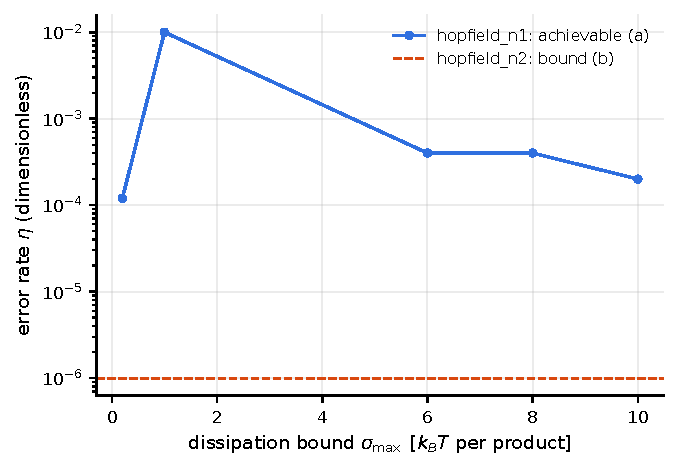
\includegraphics[width=\columnwidth]{pareto_front.pdf}\caption{Certified achievable error thresholds (dots; each dot is the threshold of one exact certificate, not an optimum) and proven lower bounds (dashed lines).}\end{figure}
\begin{figure}[t]\centering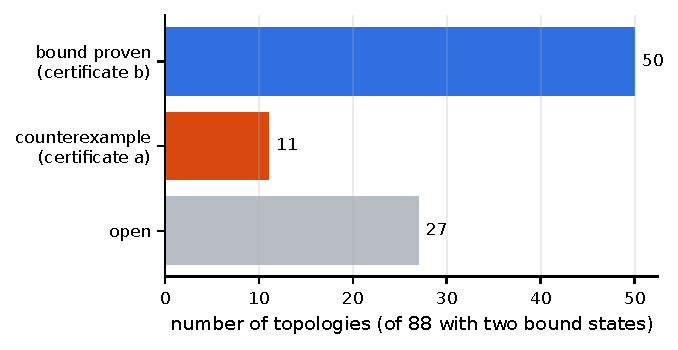
\includegraphics[width=\columnwidth]{klassifikation.pdf}\caption{Classification of the 88 non-degenerate networks with two bound states with respect to the bound $\eta \geq e^{-2\Delta}$.}\end{figure}

\bibliographystyle{unsrt}
\bibliography{references}
\end{document}
